\documentclass[10.5pt]{article}
\usepackage{amsfonts, amsmath, amssymb}
\usepackage{multirow, multicol}
\usepackage{epsfig, subfigure, subfloat, graphicx}
\usepackage{anysize, indentfirst, setspace}
\usepackage{verbatim, rotating, paralist}
\usepackage{caption, hanging}
\usepackage{pstricks, sgamevar, egameps}
\usepackage{lscape}
\usepackage{tikz}
\usepackage{hyperref}
\usetikzlibrary{shapes,arrows,backgrounds,decorations.pathmorphing,decorations.pathreplacing,calc,fadings}
% These are the key packages.  There is also sgame instead of sgamevar, but it doesn't work with beamer or other macros.
% The dcolumn package interferes with these, so you need to remove it from your preamble.
\tikzfading[name=fade out, inner color=transparent!0,
  outer color=transparent!100]
  %don't worry about this, we'll talk about it later

\title{Drawing Games and Diagrams in \LaTeX\thanks{This handout borrows heavily from the department's 2010 \LaTeX~handout authored by Dave Ohls. The 2010 handout is available at \url{https://mywebspace.wisc.edu/ohls/web/teaching.html}}}
\author{Richard Loeza\\ University of Wisconsin \\ loeza@wisc.edu}
\date{\today}

\begin{document}


\maketitle

This document introduces a number of ways to draw game matrices, decision and interaction trees, spatial models, and other diagrammatic representations of aspects of strategic behavior.  The code can look a bit dense and intimidating at first, but once you get familiar with what each command (and each part of each command) is doing, these packages provide very flexible ways to draw just about any diagram you want.   \\





\section{Strategic Form Games}

To make strategic form games, the `game' environment (using the .sgamevar package) behaves much like tabular environments (in fact, you could just use tables instead if you're sophisticated in how you manage the lines).  But using this package does incorporate a few nice features: it automatically places lines in the appropriate places, it does the alignment and dimensions for you, and it centers the player and name labels horizontally and vertically.  Syntactically, it behaves exactly like the tabular environment except:\\

\begin{compactitem}
\item You use the `figure' float instead of the `table' float.
\item The \verb+\>+ replaces \verb+&+ as the divider between cells. %Note: in the sgame package, you use & still
\item The initial operators are different - rather than \verb+\begin{tabular}{l|cc}...\end{tabular}+ it is: \\ \verb+\begin{game}{rows}{columns}[player 1 label][player 2 label][figure label]...\end{game}+ \\
\end{compactitem}

\begin{figure}[h!]
\begin{center}
\begin{footnotesize}
\begin{game}{2}{3}[1][2][]
        \> Left \> Center \> Right   \\
Up      \> 3,2  \> 4,4    \> 5,1   \\
Down    \> 0,0  \> 2,6    \> 4, 3 \\
\end{game}
\end{footnotesize}
\end{center}
\end{figure}


\begin{figure}[h]
\begin{center}
\begin{scriptsize}
\begin{game}{7}{7}[\textbf{US}][\textbf{USSR}][If you like, strategic games can be quite large]
          \> Retreat  \>  Negotiate  \> Sanctions    \> Blockade   \> Airstrike  \> Invade  \> Nuclear\\
Retreat   \> 2,2      \>  2,6        \> 1,5          \> 4,3        \> 2,3        \> 3,4     \> 3,7  \\
Negotiate \> 6,2      \>  8,8        \> 3,5          \> 3,2        \> 1,1        \> 4,0     \> 2,4  \\
Sanctions \> 5,1      \>  5,3        \> 2,2          \> 2,4        \> 0,4        \> 2,5     \> 0,1  \\
Blockade  \> 3,4      \>  2,3        \> 4,2          \> 2,2        \> 7,6        \> 4,7     \> 0,1  \\
Airstrike \> 3,2      \>  1,1        \> 4,0          \> 6,7        \> 4,4        \> 5,5     \> 0,1  \\
Invade    \> 4,3      \>  0,4        \> 5,2          \> 7,4        \> 5,5        \> 6,6     \> 0,3  \\
Nuclear   \> 7,3      \>  4,2        \> 1,0          \> 1,0        \> 1,0        \> 3,0     \> -5,-5 \\
\end{game}
\end{scriptsize}
\end{center}
\end{figure}

Most stylistic commands also work inside games. Using circles to indicate best responses is problematic because the circles tend to cut off some of the number\footnote{For those wondering: Scissors cuts paper, paper covers rock, rock crushes lizard, lizard poisons Spock, Spock smashes scissors, scissors decapitates lizard, lizard eats paper, paper disproves Spock, Spock vaporizes rock, rock crushes scissors.}.

\begin{figure}[h!]
\begin{footnotesize}
 \begin{center}
\begin{game}{5}{5}[\textbf{1}][\textbf{2}][A silly game]
       \> \large{Rock}    \> Paper   \> Scissors \> Lizard \> \textit{Spock}  \\
 \large{Rock} \> \underline{1,1}  \>  0,2  \> 2,0 \> 2,0 \> 0,2 \\
 Paper \> 2,0    \> \underline{1,1}  \> 0,2 \> 0,2 \> 2,0 \\
 Scissors \> 0,2 \> 2,0 \> \underline{1,1} \> 2,0 \> 0,2 \\
 Lizard \> 0,2  \> 2,0 \> 0,2 \> \underline{1,1} \> 2,0 \\
 \textit{Spock} \> 2,0 \> 0,2 \> 2,0 \> 0,2 \> \textcircled{1},\textcircled{1} \\
\end{game}
\end{center}
\end{footnotesize}
\end{figure}


You can cluster multiple strategic games together by including them within the same `figure' float, or by having them clustered.  Here, I used the \verb+\hspace{}+ and \verb+\vspace{}+ commands to have them spaced how I wanted.


\begin{figure}[h!]
\begin{center}
\begin{footnotesize}
\begin{game}{2}{2}[1][2][(a)]
        \> Polisci \> Econ \\
Polisci \> 4,4     \> 2,1  \\
Econ    \> 1,2     \> 3,3  \\
\end{game}\hspace{.5in}
\begin{game}{2}{2}[1][2][(c)]
             \> IR   \> Theory   \\
Comparative  \> 5,6  \> 3,3      \\
American     \> 2,3  \> 4,0      \\
\end{game}
\end{footnotesize}
\end{center}
\end{figure}
\vspace{-.3in}
\begin{figure}[h!]
\begin{center}
\begin{footnotesize}
\begin{game}{2}{2}[1][2][(b)]
        \> Dayton \> Mifflin \\
Gorham  \> -4,-2  \> -2,-5   \\
Johnson \> -1,-4  \> -3,-1   \\
\end{game}\hspace{.5in}
\begin{game}{2}{2}[1][2][(d)]
             \> Batman \> Superman \\
Luthor\>2,1  \> 3,4     \\
Joker\> 3,4  \> 2,1     \\
\end{game}
\end{footnotesize}
\end{center}
\end{figure}




\section{Extensive Form Games}
Previous versions of this workshop used the .egamesps package to create extensive form games. That package makes creating extensive games simpler, but it is less easily manipulated and is extremely fragile/prone to errors. If you are interested in using egames to make extensive form games, review the 2010 LaTeX workshop handout, available at \href{https://mywebspace.wisc.edu/ohls/web/teaching.html}{https://mywebspace.wisc.edu/ohls/web/teaching.html}.

Instead, we are going to cover how to create extensive games using the `tikzpicture' environment, from the .tikz package. The tikz package is designed for drawing in general, and is very flexible. The package can accommodate nearly any shape or arrangement you desire. The basic syntax of the coding language involves drawing a series of objects (lines, geometric shapes, text), specifying their location on a coordinate scale, and specifying the properties you'd like them to have (size, style, color, shading, special features). 


\begin{center}
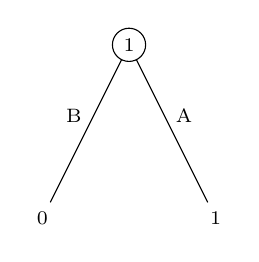
\begin{tikzpicture}[scale=1]
\draw(0,2) -- (1,0);
\draw(0,2) -- (-1,0);
\draw (.7,1.1) node{\scriptsize{A}};
\draw (-.7,1.1) node{\scriptsize{B}};
\draw(1.1,-.2) node {\scriptsize{1}};
\draw(-1.1,-.2) node {\scriptsize{0}};
\filldraw[fill=white](0,2) circle (6pt) node{\scriptsize{1}};
\end{tikzpicture}
\end{center}

What the commands are doing: \\

\begin{compactitem}
\item \verb+[scale=1]+Scales the figure with the dimensions given (in centimeters).  Increase (or decrease) the scale to expand (or shrink) the figure.
\item \verb+\draw (0,2) -- (1,0);+: Draws a straight line between coordinate points (0,2) and (1,0).
\item \verb+\draw (.7,1.1) node{\scriptsize{A}};+ Creates a node with the small text A at the coordinates (.7,1.1).
\item \verb+\filldraw[fill=white](0,2) circle (6pt) node{\scriptsize{1}};+ Creates a circle, 6 points in diameter and fills the inside white. It then creates a small 1 in the middle of the circle. Note that this will cover up anything under the filled circle. 
\end{compactitem}
\vspace{.5cm}
With tikz, the order in which objects are rendered is important. A filled circle will go over anything at the same coordinates if it is listed after those things. Note how the above figure looks when the ordering is changed.

\begin{center}
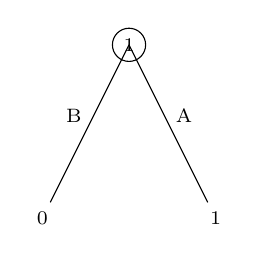
\begin{tikzpicture}[scale=1]
\filldraw[fill=white](0,2) circle (6pt) node{\scriptsize{1}};
\draw(0,2) -- (1,0);
\draw(0,2) -- (-1,0);
\draw (.7,1.1) node{\scriptsize{A}};
\draw (-.7,1.1) node{\scriptsize{B}};
\draw(1.1,-.2) node {\scriptsize{1}};
\draw(-1.1,-.2) node {\scriptsize{0}};
\end{tikzpicture}
\end{center}

Note that every line in a tikzpicture ends in a semicolon. A common error is forgetting to put one in.\\

With these basic tools, you can make games in a variety of shapes.
\begin{multicols}{2}

\begin{center}
\begin{scriptsize}
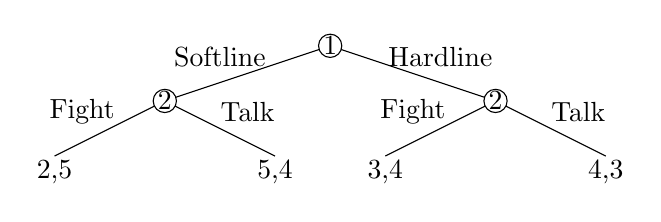
\begin{tikzpicture}[scale=.7]
\draw(7,3) -- (4,2);
\draw(7,3) -- (10,2);
\draw (5,2.8) node{Softline};
\draw (9,2.8) node{Hardline};
\draw(4,2) -- (2,1);
\draw(4,2) -- (6,1);
\draw (2.5,1.8) node{Fight};
\draw (5.5,1.8) node{Talk};
\draw(10,2) -- (8,1);
\draw(10,2) -- (12,1);
\draw (8.5,1.8) node{Fight};
\draw (11.5,1.8) node{Talk};
\filldraw[fill=white](7,3) circle (6pt) node{1};
\filldraw[fill=white](4,2) circle (6pt) node{2};
\filldraw[fill=white](10,2) circle (6pt) node{2};
\draw(2,.7) node {2,5};
\draw(6,.7) node {5,4};
\draw(8,.7) node {3,4};
\draw(12,.7) node {4,3};
\end{tikzpicture}
\end{scriptsize}
\end{center}

\begin{center}
\begin{footnotesize}
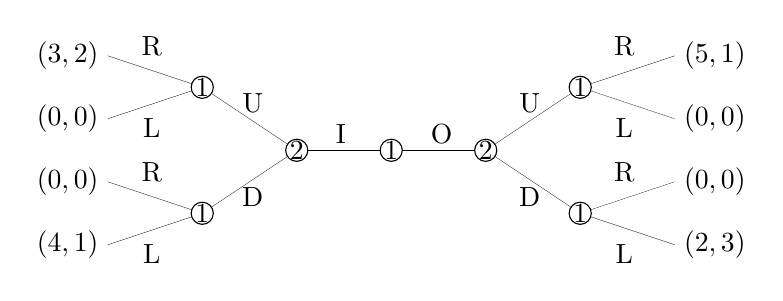
\begin{tikzpicture}[scale=.8]
\draw[ultra thin] (6,0) -- (7.5,1); 
\draw[ultra thin] (6,0) -- (7.5,-1);
\draw[ultra thin] (6,0) -- (4.5,0);
\draw[ultra thin] (3,0) -- (4.5,0);
\draw[ultra thin] (3,0) -- (1.5,1); 
\draw[ultra thin] (3,0) -- (1.5,-1);
\draw (6.7,.75) node{U};
\draw (6.7,-.75) node{D};
\draw (2.3,.75) node{U};
\draw (2.3,-.75) node{D};
\draw (3.7,.25) node{I};
\draw (5.3,.25) node{O};
\filldraw[fill=white] (6,0) circle (5pt) node {2};
\filldraw[fill=white] (3,0) circle (5pt) node {2};
\filldraw[fill=white] (4.5,0) circle (5pt) node {1};
\draw[ultra thin] (7.5,-1) -- (9,-.5) node[right]{$(0,0)$};
\draw[ultra thin] (7.5,-1) -- (9,-1.5) node[right]{$(2,3)$};
\draw (8.2,-.35) node{R};
\draw (8.2,-1.65) node{L};
\draw (8.2,.35) node{L};
\draw (8.2,1.65) node{R};
\filldraw[fill=white] (7.5,-1) circle (5pt) node {1};
\draw[ultra thin] (7.5,1) -- (9,.5) node[right]{$(0,0)$};
\draw[ultra thin] (7.5,1) -- (9,1.5) node[right]{$(5,1)$};
\filldraw[fill=white] (7.5,1) circle (5pt) node {1};
\draw[ultra thin] (1.5,1) -- (0,.5) node[left]{$(0,0)$};
\draw[ultra thin] (1.5,1) -- (0,1.5) node[left]{$(3,2)$};
\draw[ultra thin] (1.5,-1) -- (0,-.5) node[left]{$(0,0)$};
\draw[ultra thin] (1.5,-1) -- (0,-1.5) node[left]{$(4,1)$};
\draw (.7,-.35) node{R};
\draw (.7,-1.65) node{L};
\draw (.7,.35) node{L};
\draw (.7,1.65) node{R};
\filldraw[fill=white] (1.5,1) circle (5pt) node {1};
\filldraw[fill=white] (1.5,-1) circle (5pt) node {1};
\end{tikzpicture}
\end{footnotesize}
\end{center}

\begin{center}
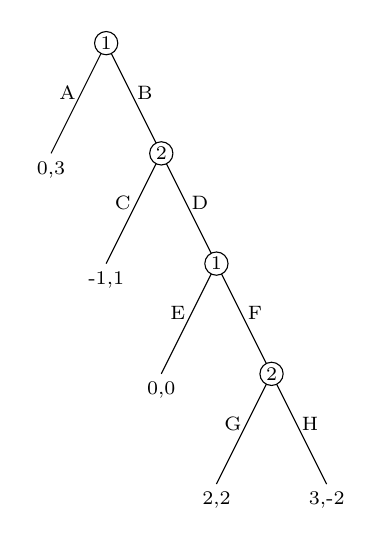
\begin{tikzpicture}[scale=.7]
\draw(5,6) -- (4,4);
\draw(5,6) -- (6,4);
\draw (4.3,5.1) node{\scriptsize{A}};
\draw (5.7,5.1) node{\scriptsize{B}};
\draw(6,4) -- (5,2);
\draw(6,4) -- (7,2);
\draw (5.3,3.1) node{\scriptsize{C}};
\draw (6.7,3.1) node{\scriptsize{D}};
\draw(7,2) -- (6,0);
\draw(7,2) -- (8,0);
\draw (6.3,1.1) node{\scriptsize{E}};
\draw (7.7,1.1) node{\scriptsize{F}};
\draw (8,0) -- (7,-2);
\draw (8,0) -- (9,-2);
\draw (7.3,-.9) node{\scriptsize{G}}; 
\draw (8.7,-.9) node {\scriptsize{H}};
\filldraw[fill=white](5,6) circle (6pt) node{\scriptsize{1}};
\filldraw[fill=white](6,4) circle (6pt) node{\scriptsize{2}};
\filldraw[fill=white](7,2) circle (6pt) node{\scriptsize{1}};
\draw(4,3.7) node {\scriptsize{0,3}};
\draw(5,1.7) node {\scriptsize{-1,1}};
\draw(6,-.3) node {\scriptsize{0,0}};
\filldraw[fill=white](8,0)  circle (6pt) node {\scriptsize{2}};
\draw(7,-2.3) node {\scriptsize{2,2}};
\draw(9,-2.3) node {\scriptsize{3,-2}};
\end{tikzpicture}
\end{center}

\end{multicols}

\begin{center}
\begin{scriptsize}
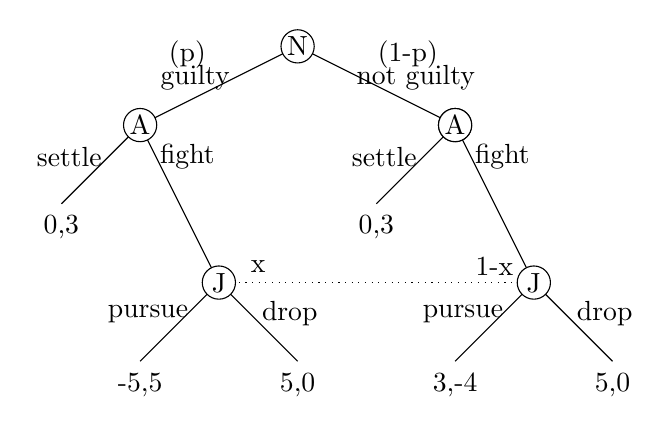
\begin{tikzpicture}[scale=1]
\draw(4,4) -- (2,3);
\draw(4,4) -- (6,3);
\draw(2.6,3.9) node{(p)};
\draw(2.7,3.6) node {guilty};
\draw(5.4,3.9) node{(1-p)};
\draw(5.5,3.6) node {not guilty};
\draw[dotted](3,1) -- (7,1);
\draw(2,3) -- (1,2);
\draw(2,3) -- (3,1);
\draw (1.1,2.6) node{settle};
\draw (2.6,2.6) node{fight};
\draw(3,1) -- (2,0);
\draw(3,1) -- (4,0);
\draw (2.1,.6) node{pursue};
\draw (3.9,.6) node{drop};
\filldraw[fill=white](4,4) circle (6pt) node{N};
\filldraw[fill=white](2,3) circle (6pt) node{A};
\filldraw[fill=white](6,3) circle (6pt) node{A};
\filldraw[fill=white](3,1) circle (6pt) node{J};
\draw(1,1.7) node {0,3};
\draw(2,-.3) node {-5,5};
\draw(4,-.3) node {5,0};
\draw(6,3) -- (5,2);
\draw(6,3) -- (7,1);
\draw (5.1,2.6) node{settle};
\draw (6.6,2.6) node{fight};
\draw(7,1) -- (6,0);
\draw(7,1) -- (8,0);
\draw (6.1,.6) node{pursue};
\draw (7.9,.6) node{drop};
\filldraw[fill=white](7,1) circle (6pt) node{J};
\filldraw[fill=white](6,3) circle (6pt) node{A};
\draw(5,1.7) node {0,3};
\draw(6,-.3) node {3,-4};
\draw(8,-.3) node {5,0};
\draw(3.5,1.2) node {x};
\draw(6.5,1.2) node {1-x};
\end{tikzpicture}
\end{scriptsize}
\end{center}
\verb+\draw[dotted](3,1) -- (7,1);+ creates a dotted line from (3,1) to (7,1).
\clearpage

\begin{landscape}
~\vspace{1in}
\begin{figure}[h!]
\begin{center}
\begin{tiny}
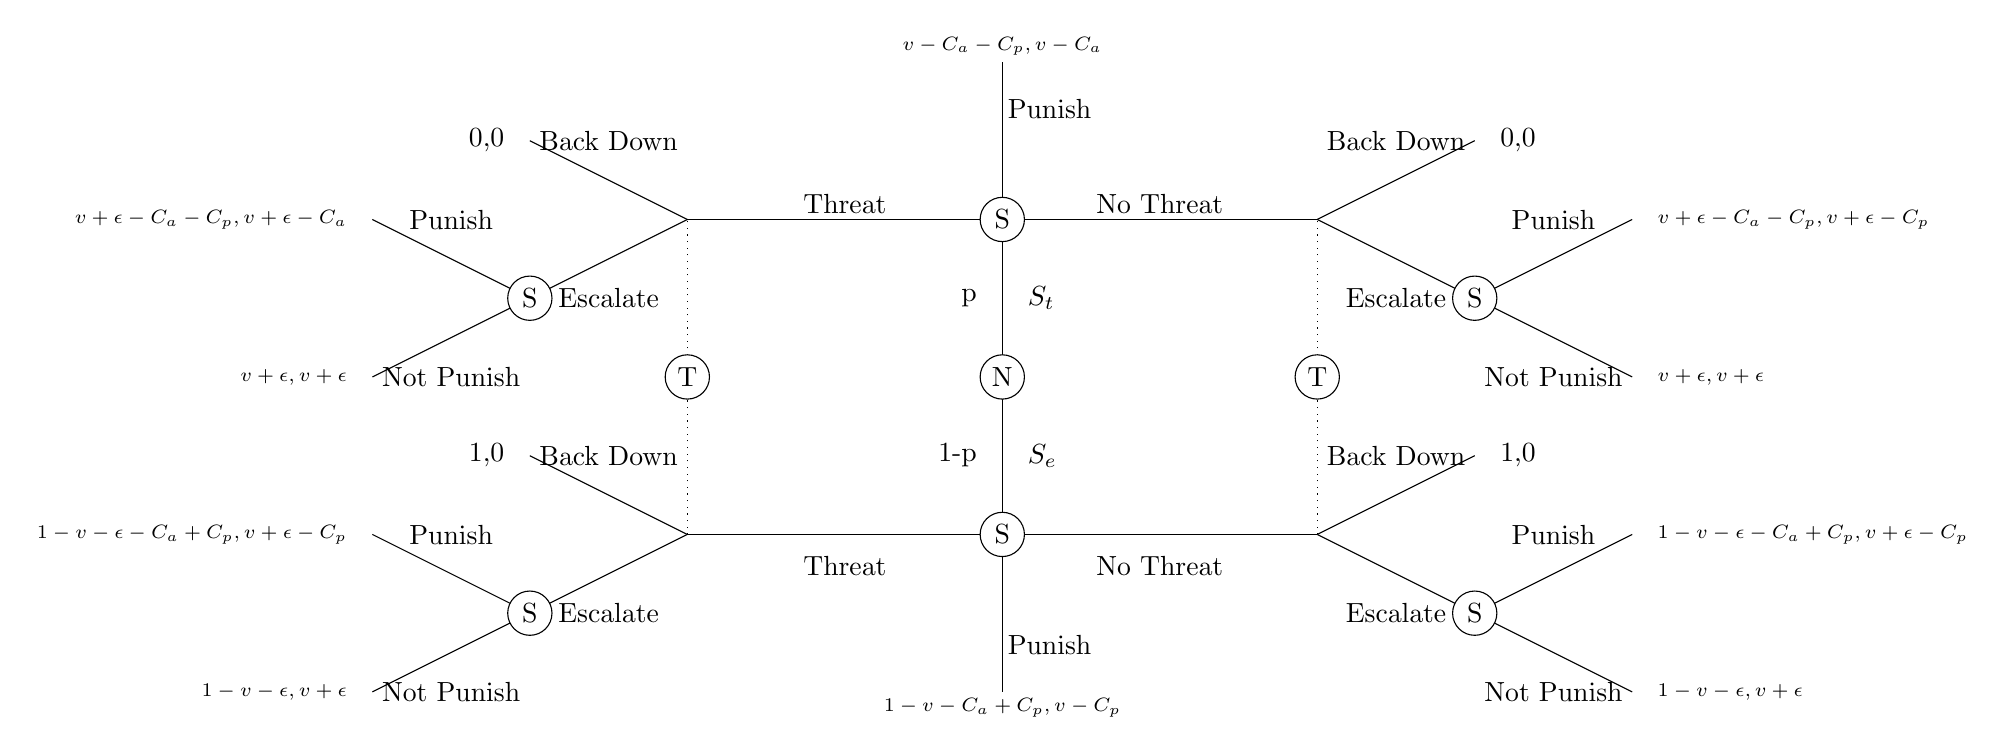
\begin{tikzpicture}[scale=2]
\draw (0,-1) -- (0,1);
\filldraw[fill=white] (0,0) circle (4pt) node {N};
\draw (0.1,0.5) node[anchor=west]{$S_t$};
\draw (0.1,-0.5) node[anchor=west]{$S_e$};
\draw (-0.1,0.5) node[anchor=east]{p};
\draw (-0.1,-0.5) node[anchor=east]{1-p};
\draw (-2,1) -- (2,1);
\draw (-2,-1) -- (2,-1);
\draw (-1,1.1) node {Threat};
\draw (1,1.1) node {No Threat};
\draw (-1,-1.2) node {Threat};
\draw (1,-1.2) node {No Threat};
\draw (0,1) -- (0,2);
\draw (0,-1) -- (0,-2);
\draw (.3,1.7) node {Punish};
\draw (.3,-1.7) node {Punish};
\draw (0,2.1) node{\scriptsize{$v-C_a-C_p, v-C_a$}};
\draw (0,-2.1) node{\scriptsize{$1-v-C_a+C_p, v-C_p$}};
\filldraw[fill=white] (0,1) circle (4pt) node {S};
\filldraw[fill=white] (0,-1) circle (4pt) node {S};
\draw[dotted] (-2,-1) -- (-2,1);
\draw[dotted] (2,-1) -- (2,1);
\filldraw[fill=white] (-2,0) circle (4pt) node {T};
\filldraw[fill=white] (2,0) circle (4pt) node {T};
\draw (-2,1) -- (-3,1.5);
\draw (-2,1) -- (-3,0.5);
\draw (-2.5,1.5) node{Back Down};
\draw (-2.5,0.5) node{Escalate};
\draw (-2,-1) -- (-3,-1.5);
\draw (-2,-1) -- (-3,-0.5);
\draw (-2.5,-0.5) node{Back Down};
\draw (-2.5,-1.5) node{Escalate};
\draw (2,1) -- (3,1.5);
\draw (2,1) -- (3,0.5);
\draw (2.5,1.5) node{Back Down};
\draw (2.5,0.5) node{Escalate};
\draw (2,-1) -- (3,-1.5);
\draw (2,-1) -- (3,-0.5);
\draw (2.5,-0.5) node{Back Down};
\draw (2.5,-1.5) node{Escalate};
\draw (3,0.5) -- (4,1);
\draw (3,0.5) -- (4,0);
\draw (3.5,-1) node{Punish};
\draw (3.5,-2) node{Not Punish};
\draw (3,-1.5) -- (4,-1);
\draw (3,-1.5) -- (4,-2);
\draw (-3.5,-1) node{Punish};
\draw (-3.5,-2) node{Not Punish};
\draw (-3,-1.5) -- (-4,-1);
\draw (-3,-1.5) -- (-4,-2);
\draw (-3.5,1) node{Punish};
\draw (-3.5,0) node{Not Punish};
\draw (-3,0.5) -- (-4,1);
\draw (-3,0.5) -- (-4,0);
\draw (3.5,1) node{Punish};
\draw (3.5,0) node{Not Punish};
\draw (3.1,1.5) node[anchor=west]{0,0};
\filldraw[fill=white] (3,0.5) circle (4pt) node{S};
\draw (3.1,-0.5) node[anchor=west]{1,0};
\filldraw[fill=white]  (3,-1.5) circle (4pt) node{S};
\draw (-3.1,1.5) node[anchor=east]{0,0};
\filldraw[fill=white]  (-3,0.5) circle (4pt) node{S};
\draw (-3.1,-0.5) node[anchor=east]{1,0};
\filldraw[fill=white]  (-3,-1.5) circle (4pt) node{S};
\draw (4.1,1) node[anchor=west]{\scriptsize{$v+\epsilon-C_a-C_p, v+\epsilon-C_p$}};
\draw (4.1,0) node[anchor=west]{\scriptsize{$v+\epsilon, v+\epsilon$}};
\draw (4.1,-1) node[anchor=west]{\scriptsize{$1-v-\epsilon-C_a+C_p, v+\epsilon-C_p$}};
\draw (4.1,-2) node[anchor=west]{\scriptsize{$1-v-\epsilon, v+\epsilon$}};
\draw (-4.1,-1) node[anchor=east]{\scriptsize{$1-v-\epsilon-C_a+C_p, v+\epsilon-C_p$}};
\draw (-4.1,-2) node[anchor=east]{\scriptsize{$1-v-\epsilon, v+\epsilon$}};
\draw (-4.1,1) node[anchor=east]{\scriptsize{$v+\epsilon-C_a-C_p, v+\epsilon-C_a$}};
\draw (-4.1,0) node[anchor=east]{\scriptsize{$v+\epsilon, v+\epsilon$}};
\end{tikzpicture}
\end{tiny}
\caption{Big Ol' Model}
\end{center}
\end{figure}
\end{landscape}
\clearpage

\section{Diagrams}

For some game theory applications, and for papers in general, you may want to draw diagrams or pictures - spatial models, functional forms, flow charts of processes, stylized examples of data, etc.  Tikz's versitility comes in handy for these more complex types of drawings as well. \\

\begin{figure}[h!]
\begin{center}
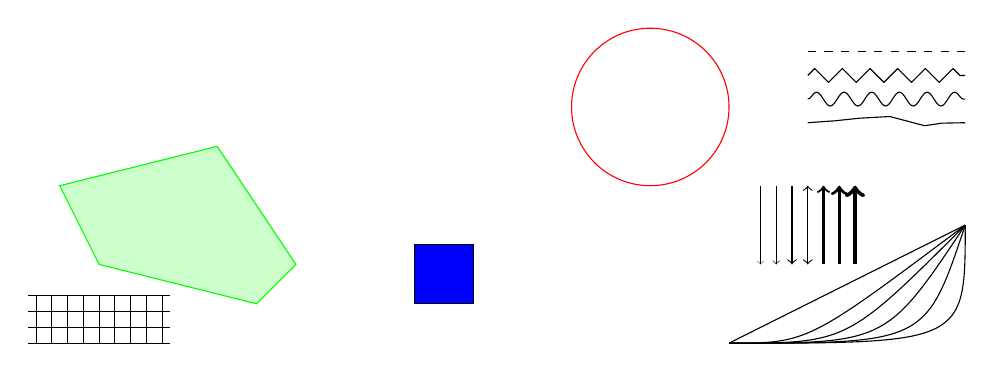
\begin{tikzpicture}[scale=1]
\draw[red] (8,3) circle(1cm);
\draw[fill=blue] (5,0.5) rectangle (5.75,1.25);
\draw[green, fill=white!80!green] (1,1) -- (3,0.5) -- (3.5,1) -- (2.5,2.5) -- (0.5,2) -- (1,1);
\draw[->, ultra thin] (9.4,2) -- (9.4,1);
\draw[->, very thin] (9.6,2) -- (9.6,1);
\draw[->, thin] (9.8,2) -- (9.8,1);
\draw[<->] (10,2) -- (10,1);
\draw[<-, thick] (10.2,2) -- (10.2,1);
\draw[<-, very thick] (10.4,2) -- (10.4,1);
\draw[<-, ultra thick] (10.6,2) -- (10.6,1);
\draw[dashed] (10,3.7) -- (12,3.7);
\draw[decorate, decoration=zigzag] (10,3.4) -- (12,3.4);
\draw[decorate, decoration=snake] (10,3.1) -- (12,3.1);
\draw[decorate, decoration=random steps] (10,2.8) -- (12,2.8);
\draw (9,0) -- (12,1.5);
\draw (9,0) .. controls (10,0) .. (12,1.5);
\draw (9,0) .. controls (10.5,0) .. (12,1.5);
\draw (9,0) .. controls (11,0) .. (12,1.5);
\draw (9,0) .. controls (11.5,0) .. (12,1.5);
\draw (9,0) .. controls (12,0) .. (12,1.5);
\draw[step=.2](0.1,0) grid (1.9,.6);
\end{tikzpicture}
\end{center}
\end{figure}

What the commands are doing: \\

\begin{compactitem}
\item \verb+\draw[red] (8,3) circle(1cm);+: Draws a circle colored red, centered at (8,3) and with radius of 1 centimeter.
\item \verb+\draw[fill=blue] (5,0.5) rectangle (5.75,1.25);+: Draws a rectangle (in this case a square) defined by corners at (5,0.5) and (5.75,1.25), and fills it blue.
\item \verb+\draw[green, fill=white!80!green] (1,1) -- (3,0.5) ... (0.5,2) -- (1,1);+: Draws a polygon region defined by the coordinates given, colored green and shaded a lighter green (80\% white, 20\% green). 
\item \verb+\draw[->, ultra thin]...+: Draws a series of lines of varying thicknesses with arrows on one or both ends.
\item \verb+\draw[dashed]+: Draws a dashed line.
\item \verb+\draw[decorate,decoration=zigzag]+: Draws an object where the lines are `decorated' or modified in some way (zigzag, snake, bumpy, random steps, text, a series of various symbols, etc).
\item \verb+\draw (9,0) .. controls (12,0) .. (12,15);+: Draws a curved line going from (9,0) to (12,1.5) with a `control point' at (12,0) that pulls it into a bend.  The line starts out toward the control point, then curves to the end point.
\item \verb+\draw[step=.2](0.1,0) grid (1.9,.6);+: Draws a grid with the specified step width covering the specified area.  Note that if you want the grid closed (like the top and bottom) you should include limits divisible by the step width, and if you want the grid open (like the left and right) you should include limits which are not.\\
\end{compactitem}

\clearpage

This can be used to create a one-dimensional spatial model with some key points highlighted and labeled:\\

\begin{figure}[h!]
\begin{center}
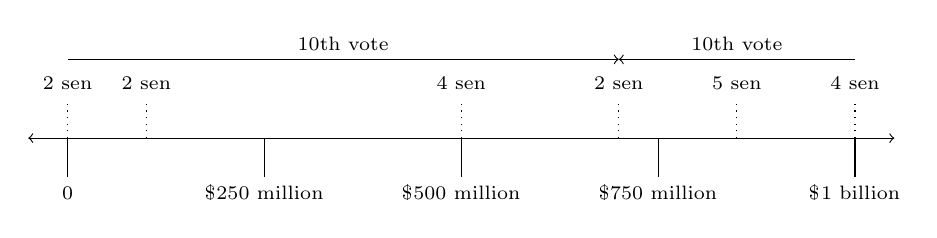
\begin{tikzpicture}[scale=1]
\draw[<->] (-.5,0) -- (10.5,0);
\draw (0,0) -- (0,-.5);
\draw (0,-.7) node{\scriptsize{0}};
\draw (2.5,0) -- (2.5,-.5);
\draw (2.5,-.7) node{\scriptsize{\$250 million}};
\draw (5,0) -- (5,-.5);
\draw (5,-.7) node{\scriptsize{\$500 million}};
\draw (7.5,0) -- (7.5,-.5);
\draw (7.5,-.7) node{\scriptsize{\$750 million}};
\draw (10,0) -- (10,-.5);
\draw (10,-.7) node{\scriptsize{\$1 billion}};
\draw (0,.7) node{\scriptsize{2 sen}};
\draw[dotted] (0,0) -- (0,.5);
\draw (1,.7) node{\scriptsize{2 sen}};
\draw[dotted] (1,0) -- (1,.5);
\draw (5,.7) node{\scriptsize{4 sen}};
\draw[dotted] (5,0) -- (5,.5);
\draw (7,.7) node{\scriptsize{2 sen}};
\draw[dotted] (7,0) -- (7,.5);
\draw (8.5,.7) node{\scriptsize{5 sen}};
\draw[dotted] (8.5,0) -- (8.5,.5);
\draw (10,.7) node{\scriptsize{4 sen}};
\draw[dotted] (10,0) -- (10,.5);
\draw[->] (0,1) -- (7,1);
\draw (3.5,1.2) node{\scriptsize{10th vote}};
\draw[<-] (7,1) -- (10,1);
\draw (8.5,1.2) node{\scriptsize{10th vote}};
\end{tikzpicture}
\end{center}
\end{figure}

\vspace{1cm}

You can extend this, along with many additional features, to draw anything else you need.  It works quite well for anything you'd like to show on a coordinate axis, such as two-dimensional spatial models or patterns over time, as well as any other drawings or flow charts you need..\\

\begin{figure}[h!]
\begin{center}
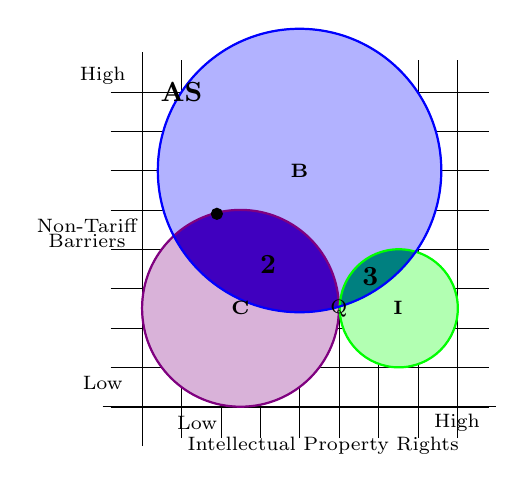
\begin{tikzpicture}[scale=1]
\draw[step=.5,black, ultra thin](-.4,-.4) grid (4.4,4.4);
\draw (-.5,0) -- (4.5,0);
\draw (-.7, 2.3) node{\scriptsize{Non-Tariff}};
\draw (-.7, 2.1) node{\scriptsize{Barriers}};
\draw (-.5, 4.2) node{\scriptsize{High}};
\draw (-.5, 0.3) node{\scriptsize{Low}};
\draw (0,-.5) -- (0,4.5);
\draw (2.3, -.5) node{\scriptsize{Intellectual Property Rights}};
\draw (4, -.2) node{\scriptsize{High}};
\draw (.7, -.2) node{\scriptsize{Low}};
\def\chinacircle{(1.25,1.25) circle(1.25cm)};
\def\indiacircle{(3.26,1.25) circle(0.75cm)};
\def\brazilcircle{(2,3) circle(1.8cm)};
\filldraw[fill=white!70!violet] \chinacircle;
\filldraw[fill=white!70!green] \indiacircle;
\filldraw[fill=white!70!blue] \brazilcircle;
\begin{scope}
    \clip \brazilcircle;
    \fill[green!50!blue] \indiacircle;
\end{scope}
\begin{scope}
    \clip \brazilcircle;
    \fill[violet!50!blue] \chinacircle;
\end{scope}
\draw[violet, thick] \chinacircle;
\draw[green, thick] \indiacircle;
\draw[blue, thick] \brazilcircle;
\draw (2.5,1.25) node{\scriptsize{Q}};
\draw (1.25,1.25) node{\scriptsize{\textbf{C}}};
\draw (3.25,1.25) node{\scriptsize{\textbf{I}}};
\draw (2,3) node{\scriptsize{\textbf{B}}};
\draw (1.6, 1.8) node{\textbf{2}};
\draw (2.9, 1.65) node{\textbf{3}};
\draw (.5, 4) node{\textbf{AS}};
\filldraw[fill=black] (.95,2.45) circle(2pt);
\end{tikzpicture}
\hspace{.5cm}
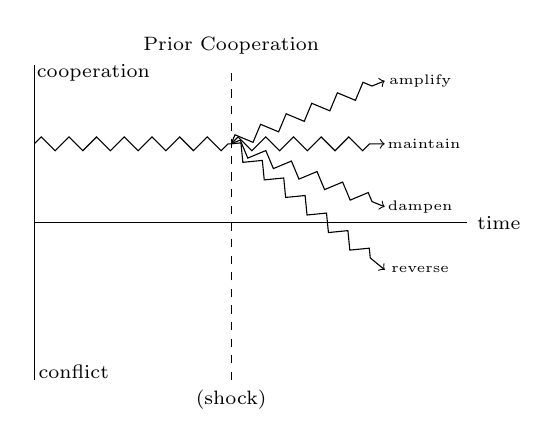
\begin{tikzpicture}[scale=1]
\draw (0,0) -- (5.5,0);
\draw (5.9,0) node{\scriptsize{time}};
\draw[dashed] (2.5,-2) -- (2.5,2);
\draw (2.5,-2.25) node{\scriptsize{(shock)}};
\draw (0,-2) -- (0,2);
\draw (.75,1.9) node{\scriptsize{cooperation}};
\draw (.5,-1.9) node{\scriptsize{conflict}};
\draw (2.5, 2.25) node{\scriptsize{Prior Cooperation}};
\draw[decorate,decoration=zigzag] (0,1.0) -- (2.5,1);
\draw[->, decorate,decoration={zigzag, post length=3}] (2.5,1) -- (4.45,1.8);
\draw[->, decorate,decoration={zigzag, post length=3}] (2.5,1) -- (4.45,1.0);
\draw[->, decorate,decoration={zigzag, post length=3}] (2.5,1) -- (4.45,.2);
\draw[->, decorate,decoration={zigzag, post length=3}] (2.5,1) -- (4.45,-.6);
\draw (4.9,1.8) node{\tiny{amplify}};
\draw (4.95,1.0) node{\tiny{maintain}};
\draw (4.9,.2) node{\tiny{dampen}};
\draw (4.9,-.6) node{\tiny{reverse}};
\end{tikzpicture}
\\ \vspace{.6cm}
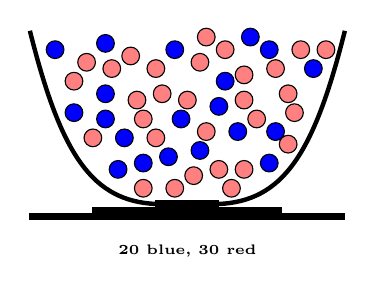
\begin{tikzpicture}[scale=.8]
\filldraw (-2.5,0) rectangle(2.5,.1);
\filldraw (-1.5,.1) rectangle (1.5,.2);
\filldraw (-.5,.2) rectangle (.5,.3);
\draw[ultra thick] (.5,.25) .. controls (1.5,.3) and (2,1) .. (2.5,3);
\draw[ultra thick] (-.5,.25) .. controls (-1.5,.3) and (-2,1) .. (-2.5,3);
\filldraw[fill=white!50!red] (-1.8,2.2) circle (4pt);
\filldraw[fill=white!50!red] (-1.6,2.5) circle (4pt);
\filldraw[fill=white!50!red] (-1.5,1.3) circle (4pt);
\filldraw[fill=white!50!red] (-.9,2.6) circle (4pt);
\filldraw[fill=white!50!red] (-.8,1.9) circle (4pt);
\filldraw[fill=white!50!red] (-.7,.5) circle (4pt);
\filldraw[fill=white!50!red] (-.5,1.3) circle (4pt);
\filldraw[fill=white!50!red] (-.7,1.6) circle (4pt);
\filldraw[fill=white!50!red] (-.5,2.4) circle (4pt);
\filldraw[fill=white!50!red] (-.2,.5) circle (4pt);
\filldraw[fill=white!50!red] (0,1.9) circle (4pt);
\filldraw[fill=white!50!red] (.2,2.5) circle (4pt);
\filldraw[fill=white!50!red] (.3,1.4) circle (4pt);
\filldraw[fill=white!50!red] (.6,2.7) circle (4pt);
\filldraw[fill=white!50!red] (.7,.5) circle (4pt);
\filldraw[fill=white!50!red] (.9,.8) circle (4pt);
\filldraw[fill=white!50!red] (.9,1.9) circle (4pt);
\filldraw[fill=white!50!red] (.9,2.3) circle (4pt);
\filldraw[fill=white!50!red] (1.1,1.6) circle (4pt);
\filldraw[fill=white!50!red] (1.4,2.4) circle (4pt);
\filldraw[fill=white!50!red] (1.6,1.2) circle (4pt);
\filldraw[fill=white!50!red] (1.6,2.0) circle (4pt);
\filldraw[fill=white!50!red] (1.7,1.7) circle (4pt);
\filldraw[fill=white!50!red] (1.8,2.7) circle (4pt);
\filldraw[fill=white!50!red] (2.2,2.7) circle (4pt);
\filldraw[fill=blue] (-2.1,2.7) circle (4pt);
\filldraw[fill=blue] (-1.8,1.7) circle (4pt);
\filldraw[fill=blue] (-1.3,1.6) circle (4pt);
\filldraw[fill=blue] (-1.3,2.0) circle (4pt);
\filldraw[fill=blue] (-1.3,2.8) circle (4pt);
\filldraw[fill=white!50!red] (-1.2,2.4) circle (4pt);
\filldraw[fill=blue] (-1.1,.8) circle (4pt);
\filldraw[fill=blue] (-1.0,1.3) circle (4pt);
\filldraw[fill=blue] (-.7,.9) circle (4pt);
\filldraw[fill=white!50!red] (-.4,2.0) circle (4pt);
\filldraw[fill=blue] (-.3,1.0) circle (4pt);
\filldraw[fill=blue] (-.2,2.7) circle (4pt);
\filldraw[fill=blue] (-.1,1.6) circle (4pt);
\filldraw[fill=white!50!red] (.1,.7) circle (4pt);
\filldraw[fill=blue] (.2,1.1) circle (4pt);
\filldraw[fill=white!50!red] (.3,2.9) circle (4pt);
\filldraw[fill=white!50!red] (.5,.8) circle (4pt);
\filldraw[fill=blue] (.5,1.8) circle (4pt);
\filldraw[fill=blue] (.6,2.2) circle (4pt);
\filldraw[fill=blue] (.8,1.4) circle (4pt);
\filldraw[fill=blue] (1.0,2.9) circle (4pt);
\filldraw[fill=blue] (1.3,.9) circle (4pt);
\filldraw[fill=blue] (1.3,2.7) circle (4pt);
\filldraw[fill=blue] (1.4,1.4) circle (4pt);
\filldraw[fill=blue] (2.0,2.4) circle (4pt);
\draw (0,-.5) node{\tiny{\textbf{20 blue, 30 red}}};
\end{tikzpicture}
\end{center}
\end{figure}


A few additional commands introduced here that are useful for diagrams with shapes that interact with each other: \\

\begin{compactitem}
\item \verb+\def\chinacircle{(1.25,1.25) circle(1.25cm)};+: `Defines' an object and names it without drawing it (yet), so you can use it in other operations and commands.
\item \verb+\filldraw[...]...+: Draws an object and fills it in at the same time, subject to commands specified in the rest of the command (or wherever the object is defined).  Note that the package draws each subsequent object on top of everything before it, so if you have two objects in the same space (e.g. a circle that is shaded in with the a label in the middle) make sure you order the draw commands such that objects on top come later.
\item \verb+\begin{scope} ... \end{scope}+: Defines the `scope' of an area for a fill command as the space where the `brazilcircle' and `indiacircle' objects overlap.\\
\end{compactitem}

\clearpage

\subsection*{Unnecessary Drawing}

	The website \href{http://www.texample.net/tikz/}{http://www.texample.net/tikz/} contains a number of more advanced tikz drawings. Check it out to see both how to make these beautiful works of art, and how to replicate them. These work especially well with your beamer presentations, where they can add much needed illustration and color to an otherwise monotonous speech. Two examples, taken from the site, are below.

\begin{figure}[h!]
\begin{center}	
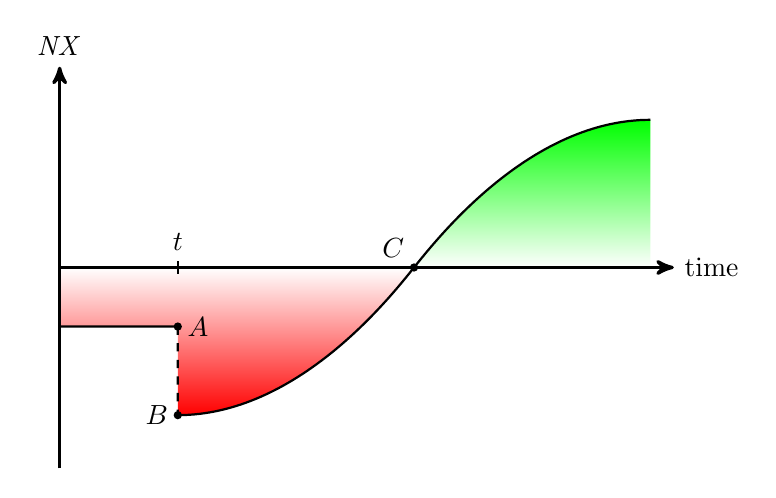
\begin{tikzpicture}[
        %We set the scale and define some styles
        scale=1.5,
        axis/.style={very thick, ->, >=stealth'},
        important line/.style={thick},
        dashed line/.style={dashed, thick},
        every node/.style={color=black,}
     ]
    % Important coordinates are defined
    \coordinate (beg_1) at (0,-.5);
    \coordinate (beg_2) at ($(beg_1)+(1,0)$);
    \coordinate (dev_1) at ($(beg_2)+(0,-.75)$);
    \coordinate (xint) at (3,0);
    \coordinate (end) at (5,1.25);

    %We make some nice shading to annotate different parts of the curve
    % Everything for x<0
    \begin{scope}
        \shade[top color=white, bottom color=red]
            ($(beg_2)+(0,.5)$) parabola bend (dev_1) (xint)
            (0,0) rectangle (beg_2);
    \end{scope}
    %  Everything for x>0
    \begin{scope}
        \shade[bottom color=white, top color=green]
            (xint) parabola bend (end) ($(end)+(0,-1.25)$);
    \end{scope}
    % axis
    \draw[axis] (0,0)  -- (5.2,0) node(xline)[right] {time};
    \draw[axis] (0,-1.7) -- (0,1.7) node(yline)[above] {$\mathit{NX}$};
    % J curve is drawn
    \draw[important line]
        (beg_1) -- (beg_2)
        (dev_1) parabola (xint)
        (xint) parabola[bend at end] (end);
    % coordinates are added
    \fill[black] (beg_2) circle (1pt) node[right] {$A$};
    \fill[black] (dev_1) circle (1pt) node[left] {$B$};
    \fill[black] (xint) circle (1pt) node[above left] {$C$};
    % The time of the devaluation is added
    \draw[dashed line] (beg_2) -- (dev_1);
    \draw[thick] (1,-1.5pt) -- (1,1.5pt) node[above] {$t$};
\end{tikzpicture}
\caption{Trade balance following a devaluation.}
\end{center}
\end{figure}
\vspace{1cm}
\begin{figure}[h!]
\begin{center}
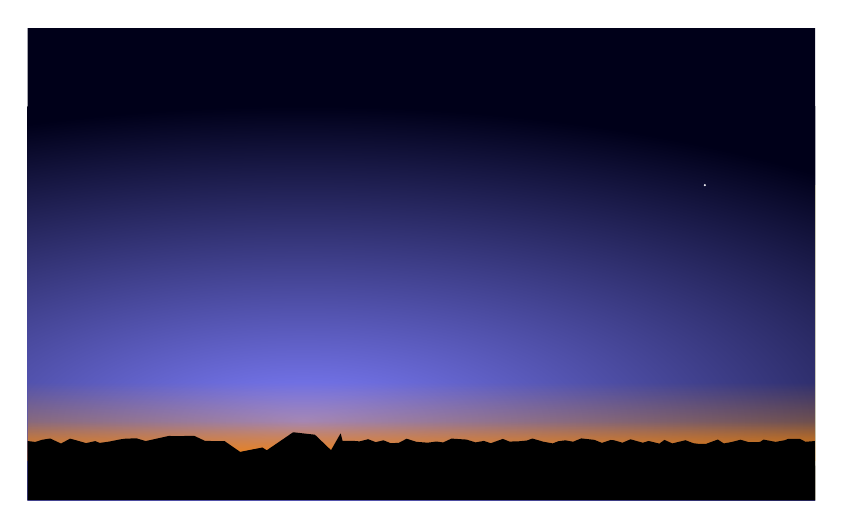
\begin{tikzpicture}
    
    \clip (-5,-3) rectangle (5,3);

    % the sky
    \fill[blue!10!black] (-6,1) rectangle (6,3);
    \fill[yellow] (-6,-3) rectangle (6,1);
    \fill[inner color=blue!50!,outer color=blue!10!black] (-12,-6) rectangle (9,2);

    % orange fadings
    \draw[draw=none] 
    [postaction={path fading=north,fill=orange!80!yellow,opacity=0.6}]
    (-7,-2.5) rectangle (7,-1.5);%
    \draw[draw=none] 
    [postaction={path fading=north,fill=orange,opacity=0.8}]
    (-7,-2.5) rectangle (7,-2);
	%This is where the /tikzfading command in the preamble came in.
	
    % the line of mountains
    \fill[black]
    decorate [decoration={random steps,segment length=3pt,amplitude=1pt}] %
    {(-5,-2.25) -- (-3.5,-2.25)}%
    decorate [decoration={random steps,segment length=5pt,amplitude=4pt}] %
    {-- (-2.5,-2.25) -- (-1,-2.25)}%
    decorate [decoration={random steps,segment length=3pt,amplitude=1pt}] %
    {-- (-1,-2.25) -- (5,-2.25)}%
    -- (5,-3) -- (-5,-3) -- (-5,-2.25);

    % a planet or a star
    \draw[color=white] (3.6,1) circle (0.005);
    
  \end{tikzpicture}  
  \caption{A Sunset!}
  \end{center}
  \end{figure}
  
 \clearpage 
  
\section{Quick and Dirty Freehand}

Finally, if you want a diagram but don't feel like wading through the coding, a quick and dirty way to do it is using a free program TeXCAD that handles these moderately well.  It works somewhat like MS Paint but much crisper, includes a few handy features for technical drawings, and it plays well with \LaTeX.  It will produce a file that you can put directly into your document using \verb+input filename.pic+ or it will give you code that will produce your picture, which you can then edit as needed.  Just to get a sense of what it can do:

\begin{center}
\input texcadsample.pic 

\begin{scriptsize}
(un-comment the picture command to display the picture if you have the file)
\end{scriptsize}
\end{center}


% NOTE: If this file is failing to compile, check if you're missing this file from the directory.  If that's the issue, either get the picture or comment-out the bit of code above.



\section{References}

The .sgamevar and .egameps packages were written by Martin Osborne, an economist at the University of Toronto, so the best resource for them is his website: \href{http://www.economics.utoronto.ca/osborne/latex/}{http://www.economics.utoronto.ca/osborne/latex/}.  The sgame.pdf and egame.pdf guide documents are particularly useful, both for debugging and for discovering more advanced features of the packages. \\

The .tikz and .pgf packages were designed by Till Tantau, a computer scientist at the University of L\"{u}beck.  The best resource for learning how it works is his extensive online manual, available at \href{http://www.ctan.org/tex-archive/graphics/pgf/base/doc/generic/pgf/pgfmanual.pdf}{http://www.ctan.org/tex-archive/graphics/pgf/base/doc/generic/pgf/pgfmanual.pdf}.  It is 560 pages long, but fortunately has a table of contents and an index and is searchable.  Most of the information you might want about how to do various things is in the `I. Tutorials and Guidelines' section, which is very user-friendly (and surprisingly funny).  There are also examples of code for all sorts of fun stuff in tikz at \href{www.texample.net}{www.texample.net}. \\

TeXCad is available for free download at \href{http://texcad.sourceforge.net/}{http://texcad.sourceforge.net/}.\\

\end{document} 

